\subsection{Conic Sections}
Conic sections include four distinct shapes: circles, ellipses, parabolas, and hyperbolas. They are called conic sections because they can be formed from cutting a cone in different ways.\\
\centerline{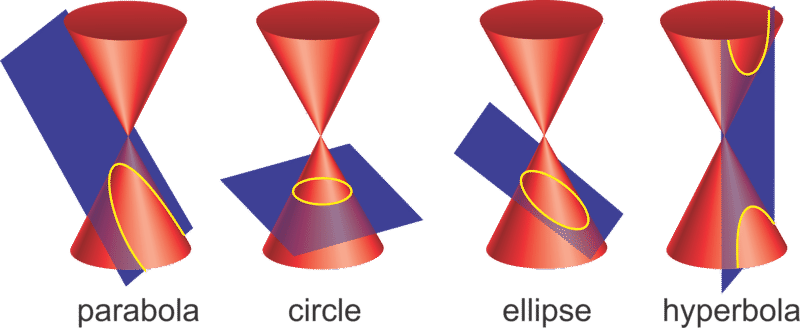
\includegraphics[scale=0.5]{PreCalcPictures/ConicSections.png}}

\subsubsection{Circles}
The standard equation for a circle is $(x+h)^2+(y-k)^2=r^2$ where the point $(h,k)$ is where the center of the circle is located and $r$ is the radius of the circle.\\
If given the equation of a circle in expanded form, you can complete the square for both $x$ and $y$ to change it to standard form.\\
\begin{align*}
    \text{Ex: } &x^2-2x+y^2+4y-4=0\\
    &(x^2+2x+1)+(y^2+4y+4)-4=1+4\\
    &(x-1)^2+(y+2)^2=9
\end{align*}

\subsubsection{Ellipses}
An ellipse is a circular object with two radii of different length.\\
Terminology:
\begin{itemize}
    \item The major axis is the longer axis (twice the length of the longer radius)
    \item The minor axis is the shorter axis (twice the length of the shorter radius)
    \item The vertices are the two points on either end of the major axis
    \item The co-vertices are the two points on either end of the minor axis
    \item The foci of an ellipse are two whose sum of distances from any of point on the ellipse is always the same. They lie on the major axis and are equidistant away from the origin.
    \item The distance between each focus and the center is called the focal length $f$ where $f^2=p^2-q^2$ where $p$ is the major radius and $q$ is the minor radius.
\end{itemize}
The standard equation for an ellipse is $\dfrac{(x-h)^2}{a^2}+\dfrac{(y-k)^2}{b^2}=1$ where t $(h,k)$ is the center point, $a$ is the horizontal axis, $b$ is the vertical radius.

\subsubsection{Parabolas}
Parabolas can be viewed as the set of all points whose distance from a certain point (the focus) is equal to their distance from a certain line called the directrix. The focus (point $(a,b)$) will always be the same distance away from the directrix (line $y=k$) along the curve of the parabola.\\
\centerline{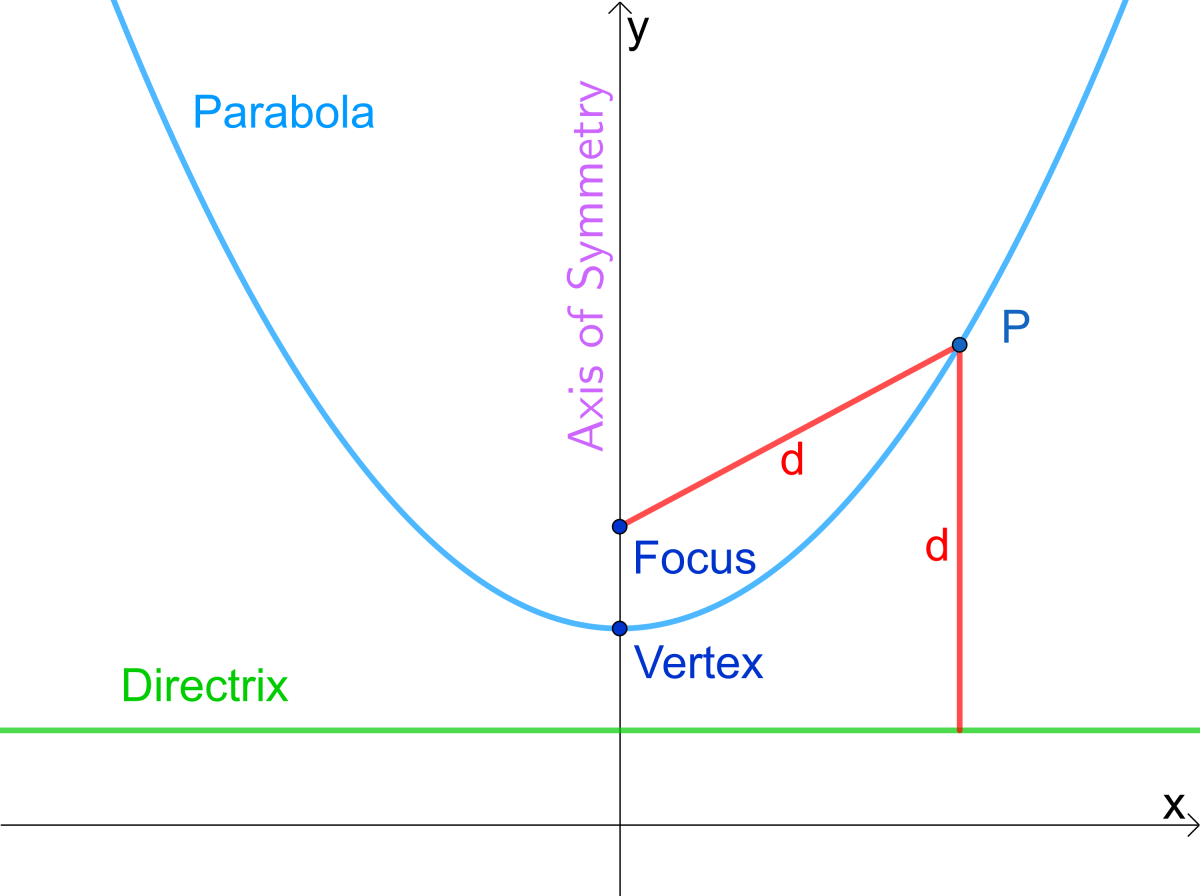
\includegraphics[scale=1.2]{PreCalcPictures/ParabolaConic.png}}
The equation of a parabola can be derived from the location of the focus and directrix using the equation $y=\dfrac{(x-a)^2}{2(b-k)}+\dfrac{b+k}{2}$\\
The location of the focus and directrix can be found from the equation of a quadratic by working backwards with the same formula.\\
Ex: $y=2(x-1)^2+4\Ra a=1$\\
\begin{align*}
    &2=\frac{1}{2(b-k)} &4=\frac{b+k}{2}\\
    &b-k=\frac{1}{4} &b=8-k\\
    &\frac{1}{4}=8-2k &\\
    &k=\frac{31}{8}\\
    &8-\frac{31}{8}=b\\
    &b=\frac{33}{8}
\end{align*}

\subsubsection{Hyperbolas}
There are two cases of hyperbolas defined by two slightly different equations: $\dfrac{(x-h)^2}{a^2}-\dfrac{(y-k)^2}{b^2}=1$ or $\dfrac{(y-k)^2}{b^2}-\dfrac{(x-h)^2}{a^2}=1$\\
If the x-term is positive, the hyperbola will open up to the side. if the y-term is positive, the hyperbola will open up.\\
$a$ is always associated with the x-term and $b$ is always associated with the y-term.\\
The point $(h,k)$ will be the center of the hyperbolas and the point $a$ or $b$ determines how far away the vertices of the hyperbola will be from its center. Each hyperbola will have 2 diagonal asymptotes that meet in its center. The slopes of the asymptotes will always be $m_{asym}=\pm\frac{b}{a}$\\
\centerline{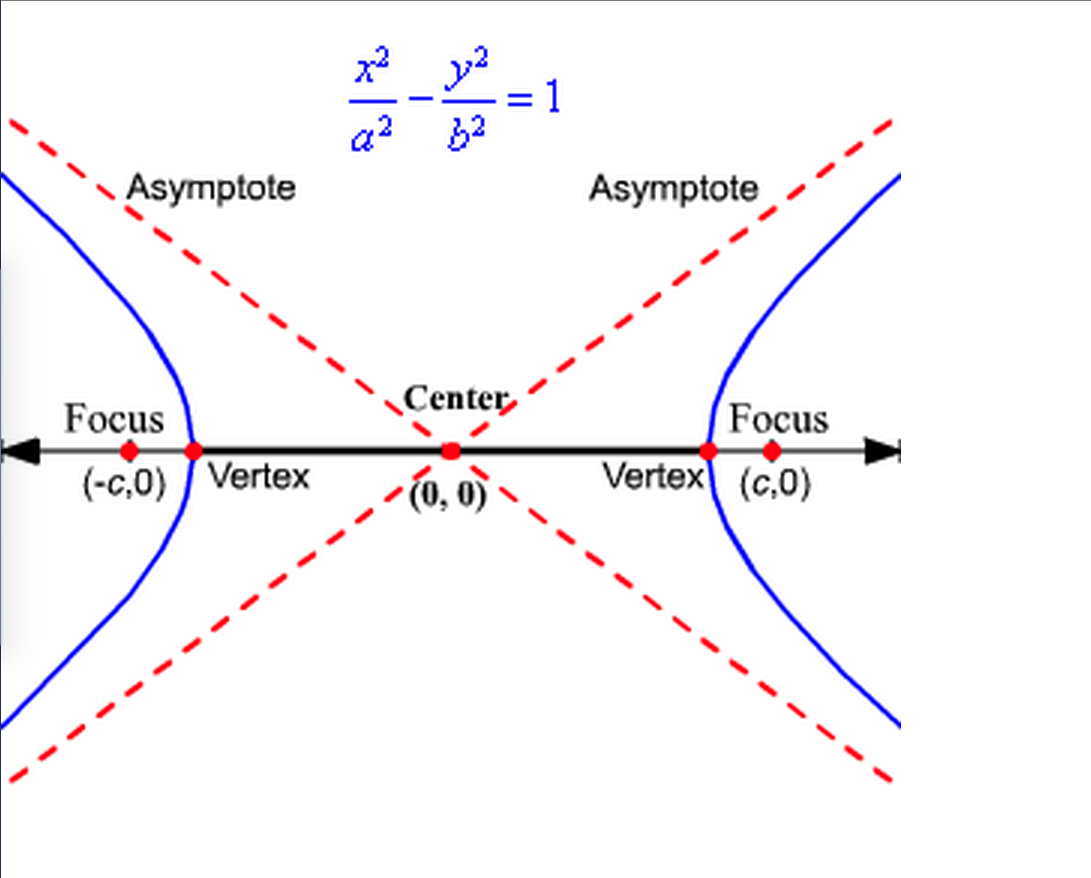
\includegraphics[scale=0.3]{PreCalcPictures/HyperbolaGraph.png}}
The difference from each focus to a point on the hyperbola will always be a constant $|d_1-d_2|=C$. If it opens horizontally, it will be $|d_1-d_2|=2a$ and if it opens vertically, it will be $|d_1-d_2|=2b$. The distance from each focus to the center of the hyperbola is $f^2=a^2+b^2$.